\section{Problem Statement and Interactive Analysis Process Design}
\label{sec:analysis_process}
Analysis of public behavior, such as how people prepare and respond to disasters, plays an important role in crisis management, disaster response, and evacuation planning. 
Recently, social media becomes popular and people utilize it for communications not only in their daily lives, but also in abnormal disastrous situations.
Thus, Location-based Social Networks services offer a new opportunity for enhancing situational awareness during disaster events.
Unfortunately, collecting relevant data can be costly and finding meaningful information from the huge volume of social media data is very challenging.
%However, the huge volume of the data is another challenging issue in analyzing and evaluating the data.
Therefore, there is a need for an advanced tool to analyze such massive (\textquotedblleft big\textquotedblright) streaming data and aid in examining the analysis results to better understand situations more efficiently.

\begin{figure}[tb]
%\centering
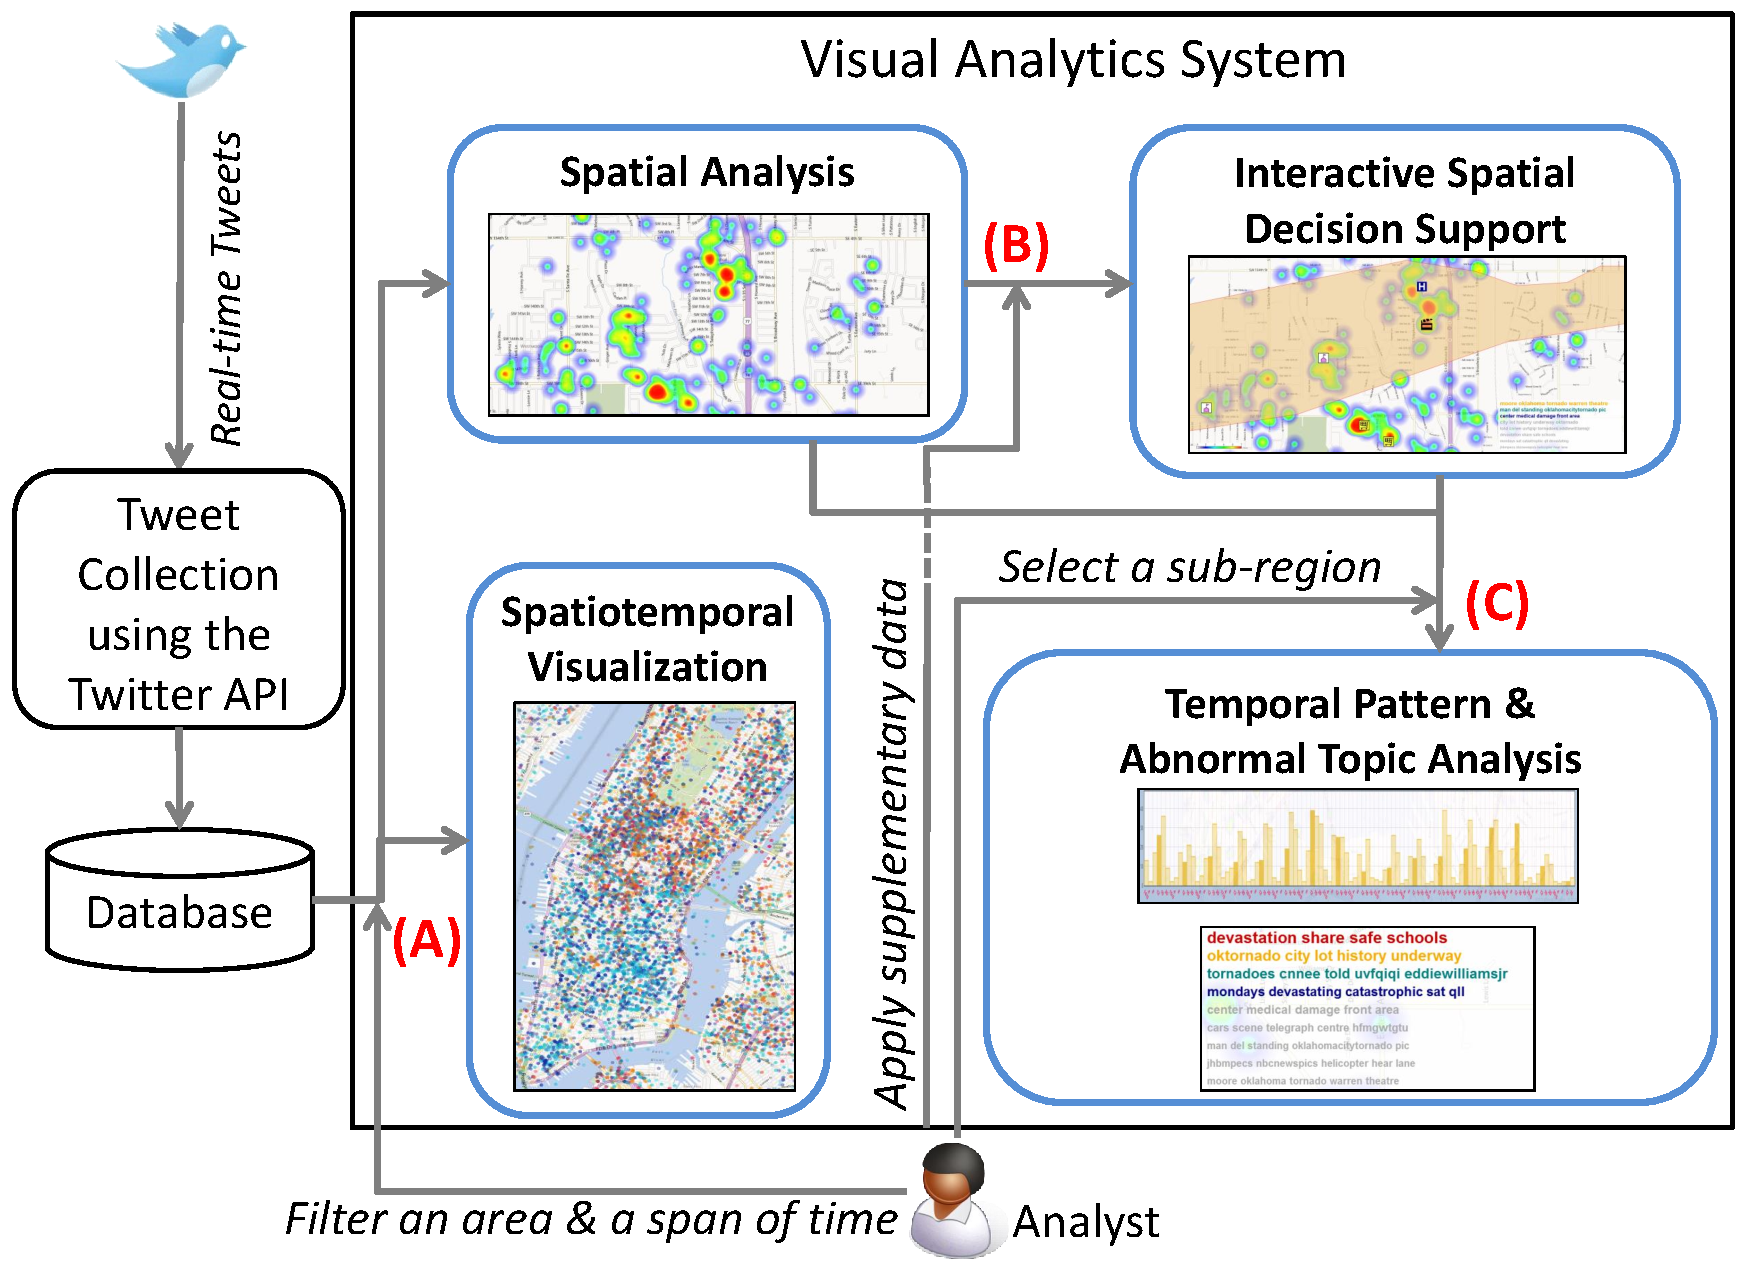
\includegraphics[width=1.0\linewidth]{System_v7}
\caption{Overview of our interactive analysis scheme for public behavior analysis using social media data.}
\label{fig:analysis_process}
%\vspace{-0.4cm}
\end{figure}

Our proposed visual analytics approach provides multiple analysis methods: spatial analysis, spatial decision support, temporal pattern analysis, abnormal topic analysis, and interactive spatiotemporal visualization as shown in Figure~\ref{fig:analysis_process}.
In our system, all methods are tightly integrated based on a user-centered design in order to enhance the ability to analyze huge social media data (Figure~\ref{fig:analysis_process}~(A, B, C)).
Our Tweet collection component obtains real-time Tweets using the Twitter API\textemdash to collect about 2.2 million geotagged Tweets within the United States per day.
In general for spatial analysis, the required accuracy of the geocoordinate depends upon the required level of location granularity.
The data, however, is generated by very reliable GPS and software.
%We can be reasonably certain about their accuracy
We can be reasonably certain about the data accuracy as illustrated in~\cite{TWITTER:2013:GOT}.
For the temporal accuracy of Tweets, we use the time when each Tweet is created. 
Therefore, it is highly accurate if the time setting of the device posting a Tweet is correct.
This large volume of data is stored in our database in order to maintain and track the history of the Twitter stream.
%The analyst can select an area and a timespan to be analyzed.
Our system allows the analysts to query Tweets with a specific area and time span condition (Figure~\ref{fig:analysis_process}~(A)).
%The initially selected spatiotemporal context of Twitter messages is represented by two different analytics components, such as spatial analysis and spatiotemporal visualization.
The initially selected spatiotemporal context of Tweets can be represented by two different analytics components: spatial analysis and spatiotemporal visualization.
Spatial analysis allows the analysts to examine the overall distribution of Twitter users and discover hotspots where relatively more Twitter users post Tweets.
The analysts are able to add supplementary information (infrastructure locations, tornado paths) on top of current information representing outcomes in order to better understand events and increase situational awareness (Figure~\ref{fig:analysis_process}~(B)).
Furthermore, the analysts can select a sub-region within the initial area, so that he can analyze the temporal patterns of the number of Twitter users and extract abnormal topics from the text messages in the selected region (Figure~\ref{fig:analysis_process}~(C)).
In addition, our interactive spatiotemporal visual analytics provides a single view representation for the analysis of both aspects: spatial and temporal characteristics of Tweets at the same time.


\section{Spatiotemporal Analysis}
\label{sec:body}

%Since many social media channels provide time-referenced geographic data, traditional techniques for spatiotemporal zooming and filtering can easily be applied to explore social media data.
%However, as the volume of the data exceed the boundaries of human evaluation capabilities and even normal computing performance, it is almost impossible to perform a straightforward qualitative analysis of the data.
%Therefore, the task for examining and determining whether the extracted result is meaningful is still challenging.
%In order to address the issues, traditional visualization approaches have to be enhanced with more interactive, scalable, and verifiable techniques, helping analysts to extract, isolate, and examine the results interactively.
In this work, we present a visual analytics approach to handle the vast amount of microblog data such as Twitter messages, provide interactive spatiotemporal analysis, and enable the use of multiple types of supplementary spatial infrastructure information for spatial decision support.
%combinational analysis of social media with different types of spatial data 
Analysts select an initial spatiotemporal context of Tweets to be represented in the visualization to serve as a basis for analysis. 
They can also perform the interactive spatiotemporal queries that load the relevant datasets from a larger database.

%in order to examine and verify the results.
%For the public behavior analysis in disasters, however, finding meaningful information from social media is challenging, since data volumes have increased beyond the capabilities of manual evaluation.
%Even though we extract certain information from the data set, it is not always easy to determine whether the result is meaningful.
%Thus, there is a need for advanced tools to handle such big data and even aid in examining the results in order to understand the situations and glean investigative insights.
%In this paper, we present an interactive visual analytics tool for spatiotemporal social media data analysis to improve emergency management, disaster preparedness and evacuation planning by allowing to identify spatiotemporal differences between emergency and normal situations, and analyze spatial relationship between location-based public behavior and locations of multiple types of infrastructures.




\subsection{Spatial Analysis}
\label{sec:spatial_analysis}
%
Social media embedding geo-location information into the data is extremely useful in analyzing location-based public behaviors.
Such spatial analysis, therefore, is important in order to manage and prepare plans for disaster and emergency situations.
%The spatial characteristics together with heterogeneous information can assist in disaster management and migrating hazards where the problems have spatial components~\cite{Andrienko:2007:GAS}.
%In this section, we present how our system supports spatial decision-making by combining different types spatial data: location-based microblog data and spatial infrastructure data.

\begin{figure}[htb]
\centering
%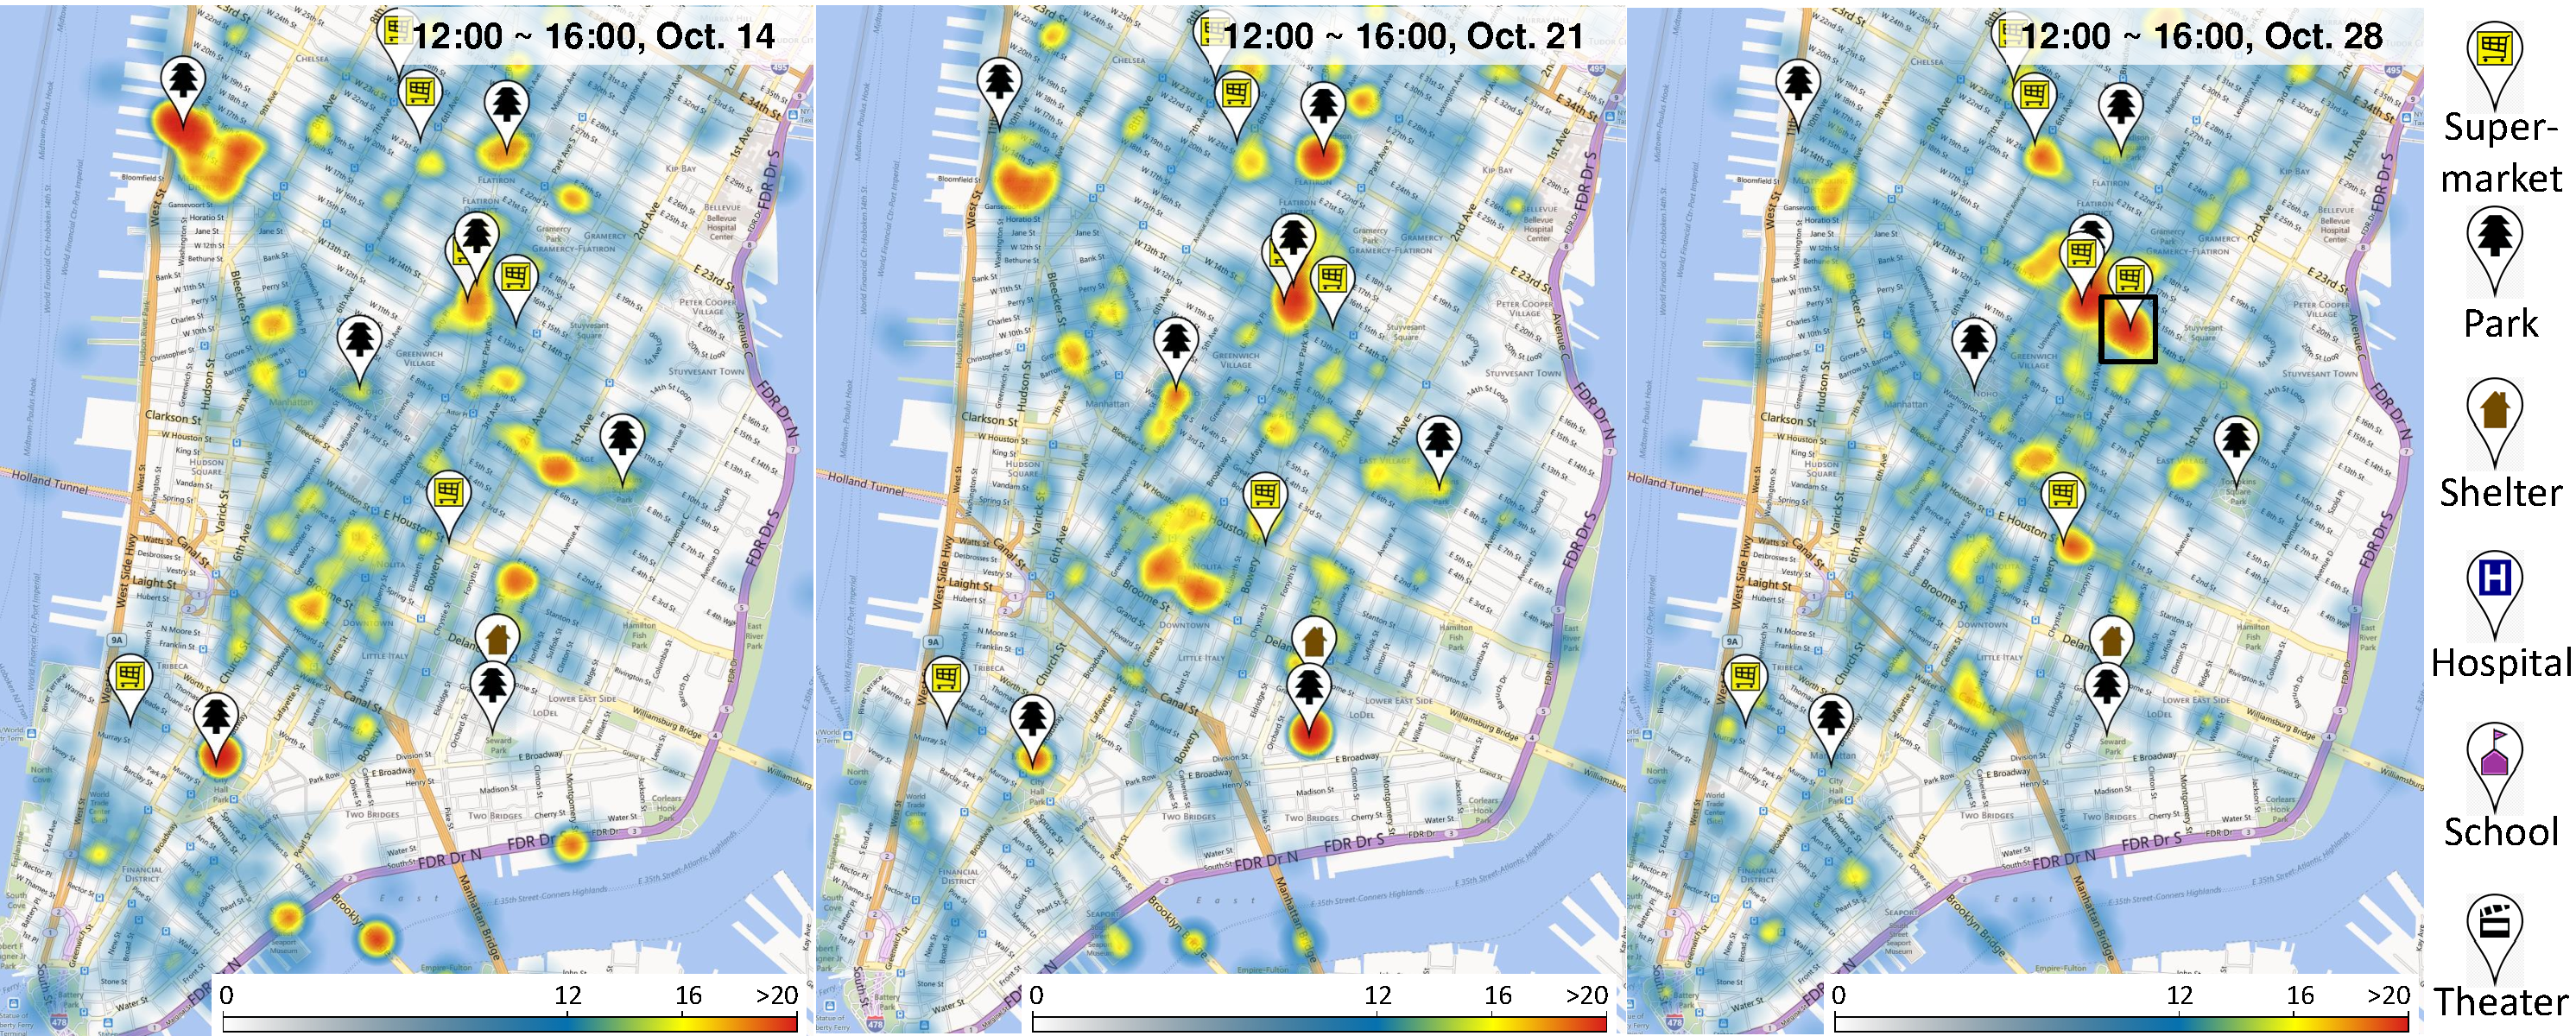
\includegraphics[width=0.9\linewidth]{heatmap_manhattan_v3}
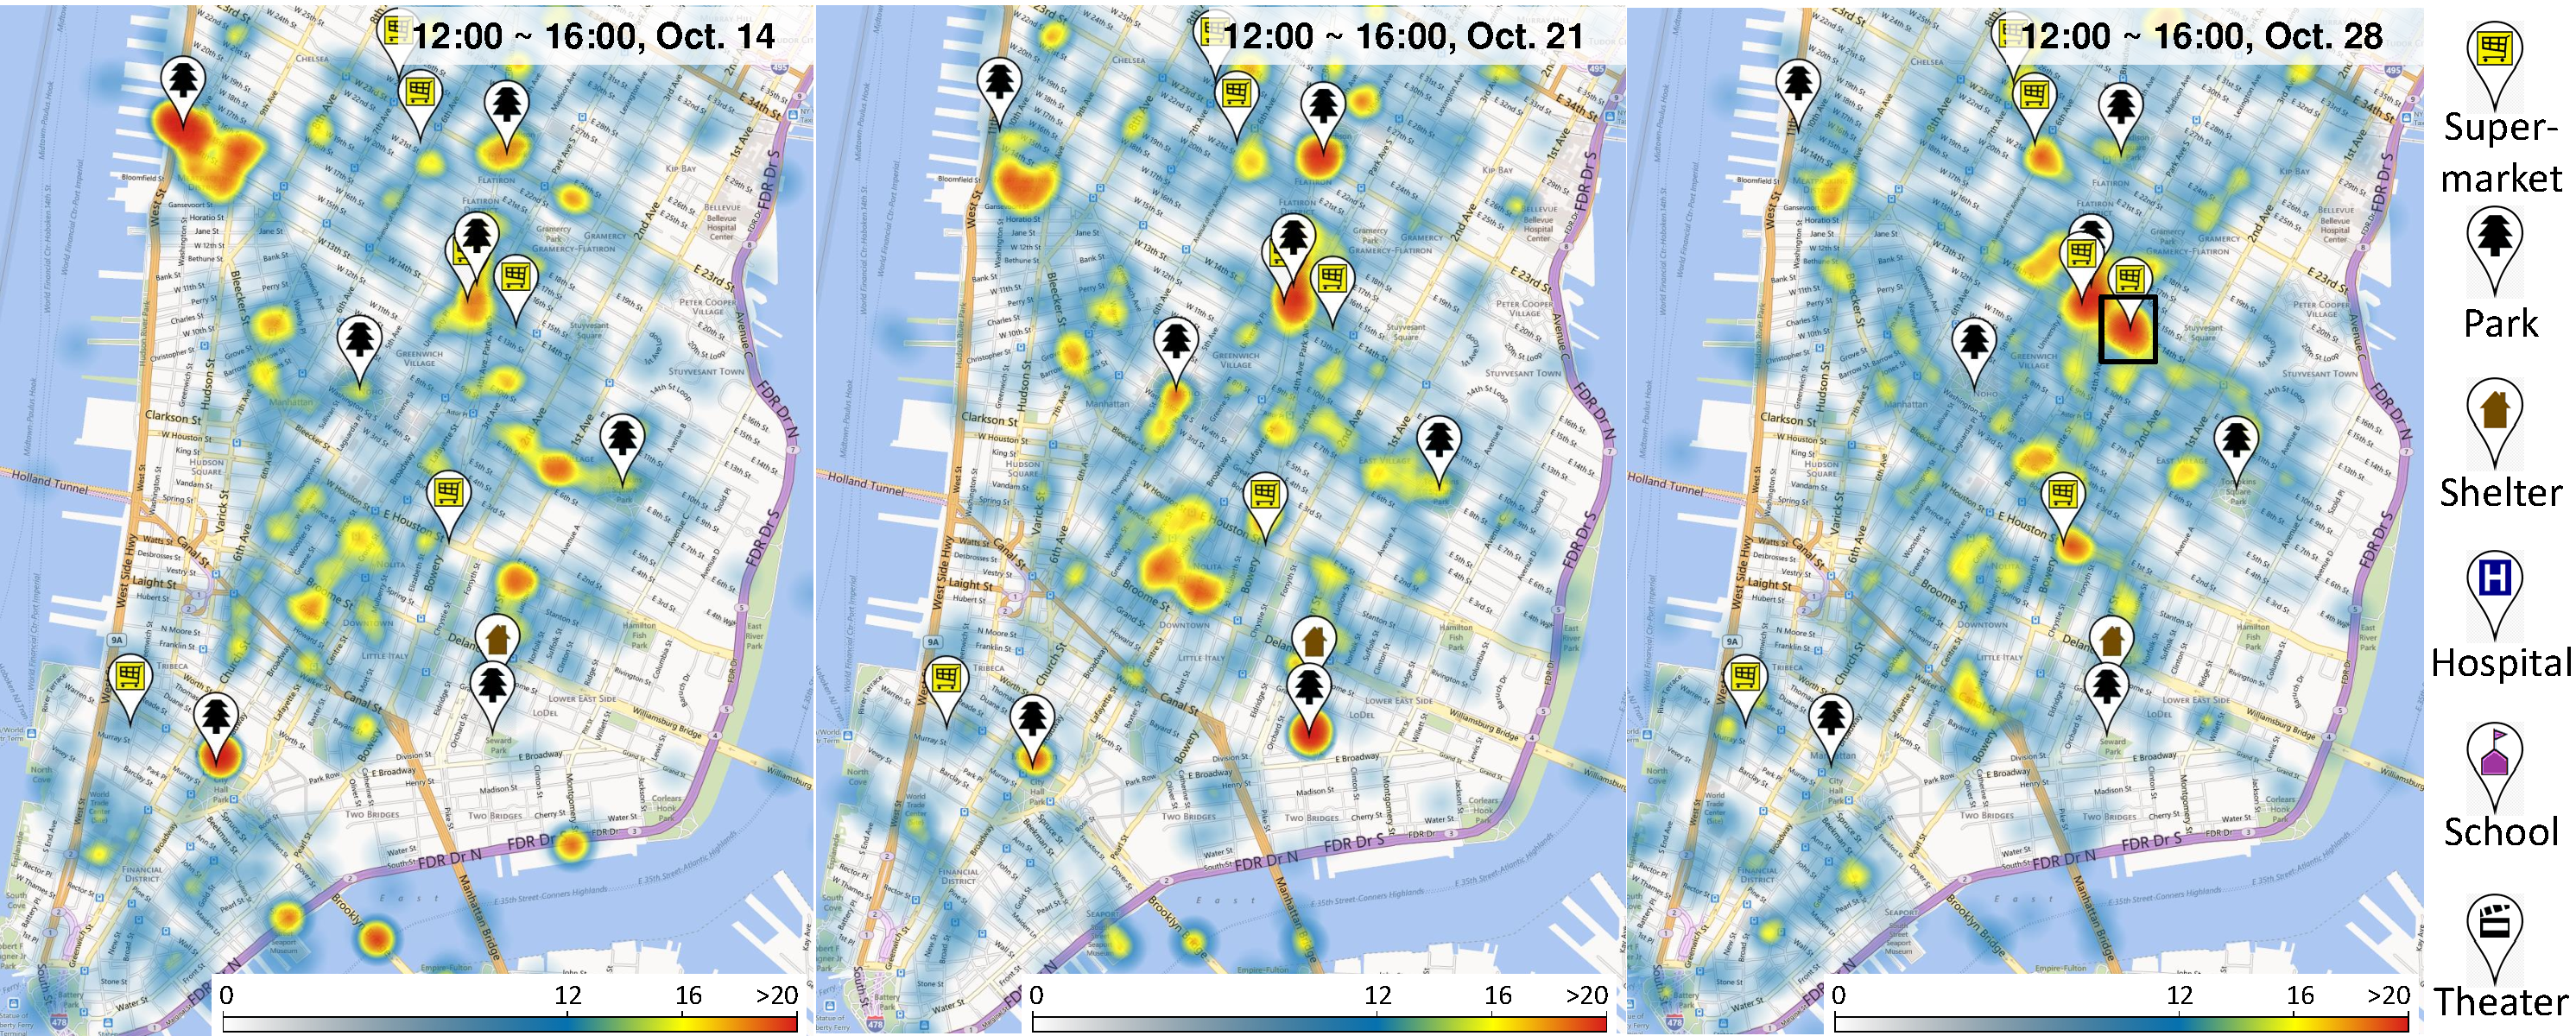
\includegraphics[width=1.0\linewidth]{heatmap_manhattan_v3}
\caption{Spatial user-based Tweet distribution in the Manhattan area in New York City during four hours right after the evacuation order (from 12:00 PM to 4:00 PM on October 28th, 2012 (Right)). Previous distribution of Tweets on 14th (Left) and 21st (Center).}
\label{fig:heatmap_manhattan}
%\vspace{-0.4cm}
\end{figure}

In late October in 2012, a massive hurricane, Sandy, devastated Northeastern United States~\cite{WKP:2012:SANDY}.
Due to the severeness of the hurricane,  on October 28th in 2012, the New York City Authorities ordered residents to leave some low-lying areas\textemdash the mandatory evacuation zones (red color) are shown in Figure~\ref{fig:spatiotemporal} (Right).
%Shelters were opened in the morning on October 28th ahead of the storm approaching the eastern third of the United States \-- the mandatory evacuation zones (red color) are shown in Figure~\ref{fig:spatiotemporal} (Right).
We investigate an area of Manhattan, since the area is the most populated and severely damaged.
Through the map view in our system, analysts navigate to the Manhattan area in New York City and filter Tweets posted within the area. 
%appearing in the view during two weeks before and after October 28th.
Initially we tried to reveal public movement flows during the disaster event, but the movement patterns were too complicated to find meaningful flows due to movement randomness and the visual clutter of the flows.
Then, we examined the spatial distribution of the users for specific time frames.
Based on our experiments, a geospatial heatmap was useful for an overview of the spatial distribution and for trend approximation.
We utilize a divergent color scheme to generate the heatmap, where saturated colors are used for the data distribution to avoid any confusion from the color scheme from the desaturated colormap of the background map.
Analysts can specify a threshold range to emphasize hotspots, where the upper bound is mapped to a red color and the lower bound to a yellow color.
Additionally, the blue color is mapped by the analysts to the value of the overall distribution of Twitter users.
In Figure~\ref{fig:heatmap_manhattan}, we show three heatmaps of spatial user-based Tweet distribution from 12:00 PM to 4:00 PM on October 14th (Left), 21st (Center), and 28th (Right).
In this work, we use the number of Twitter users instead of the number of Tweets for the heatmap generations to properly reflect the flow of evacuation unbiased by personal Tweet activity or behavior of individual users, since some enthusiastic Twitter users generate a large number of Tweets at the same location during a short time period (more than 20 Tweets per hour).
The heatmaps in Figure~\ref{fig:heatmap_manhattan} (Left and Center) represent normal situations of Twitter user distribution in the Manhattan area, and the heatmap (Right) shows the situation right after the evacuation order that was announced at 10:30 AM on October 28th, 2012.
This standard heatmap visualization allows analysts to explore the spatial pattern of Twitter users for any specified time period.
In Section~\ref{sec:spatial_decision_support}, we will provide further analysis for the spatial decision support.

\begin{figure}[tbh]
\centering
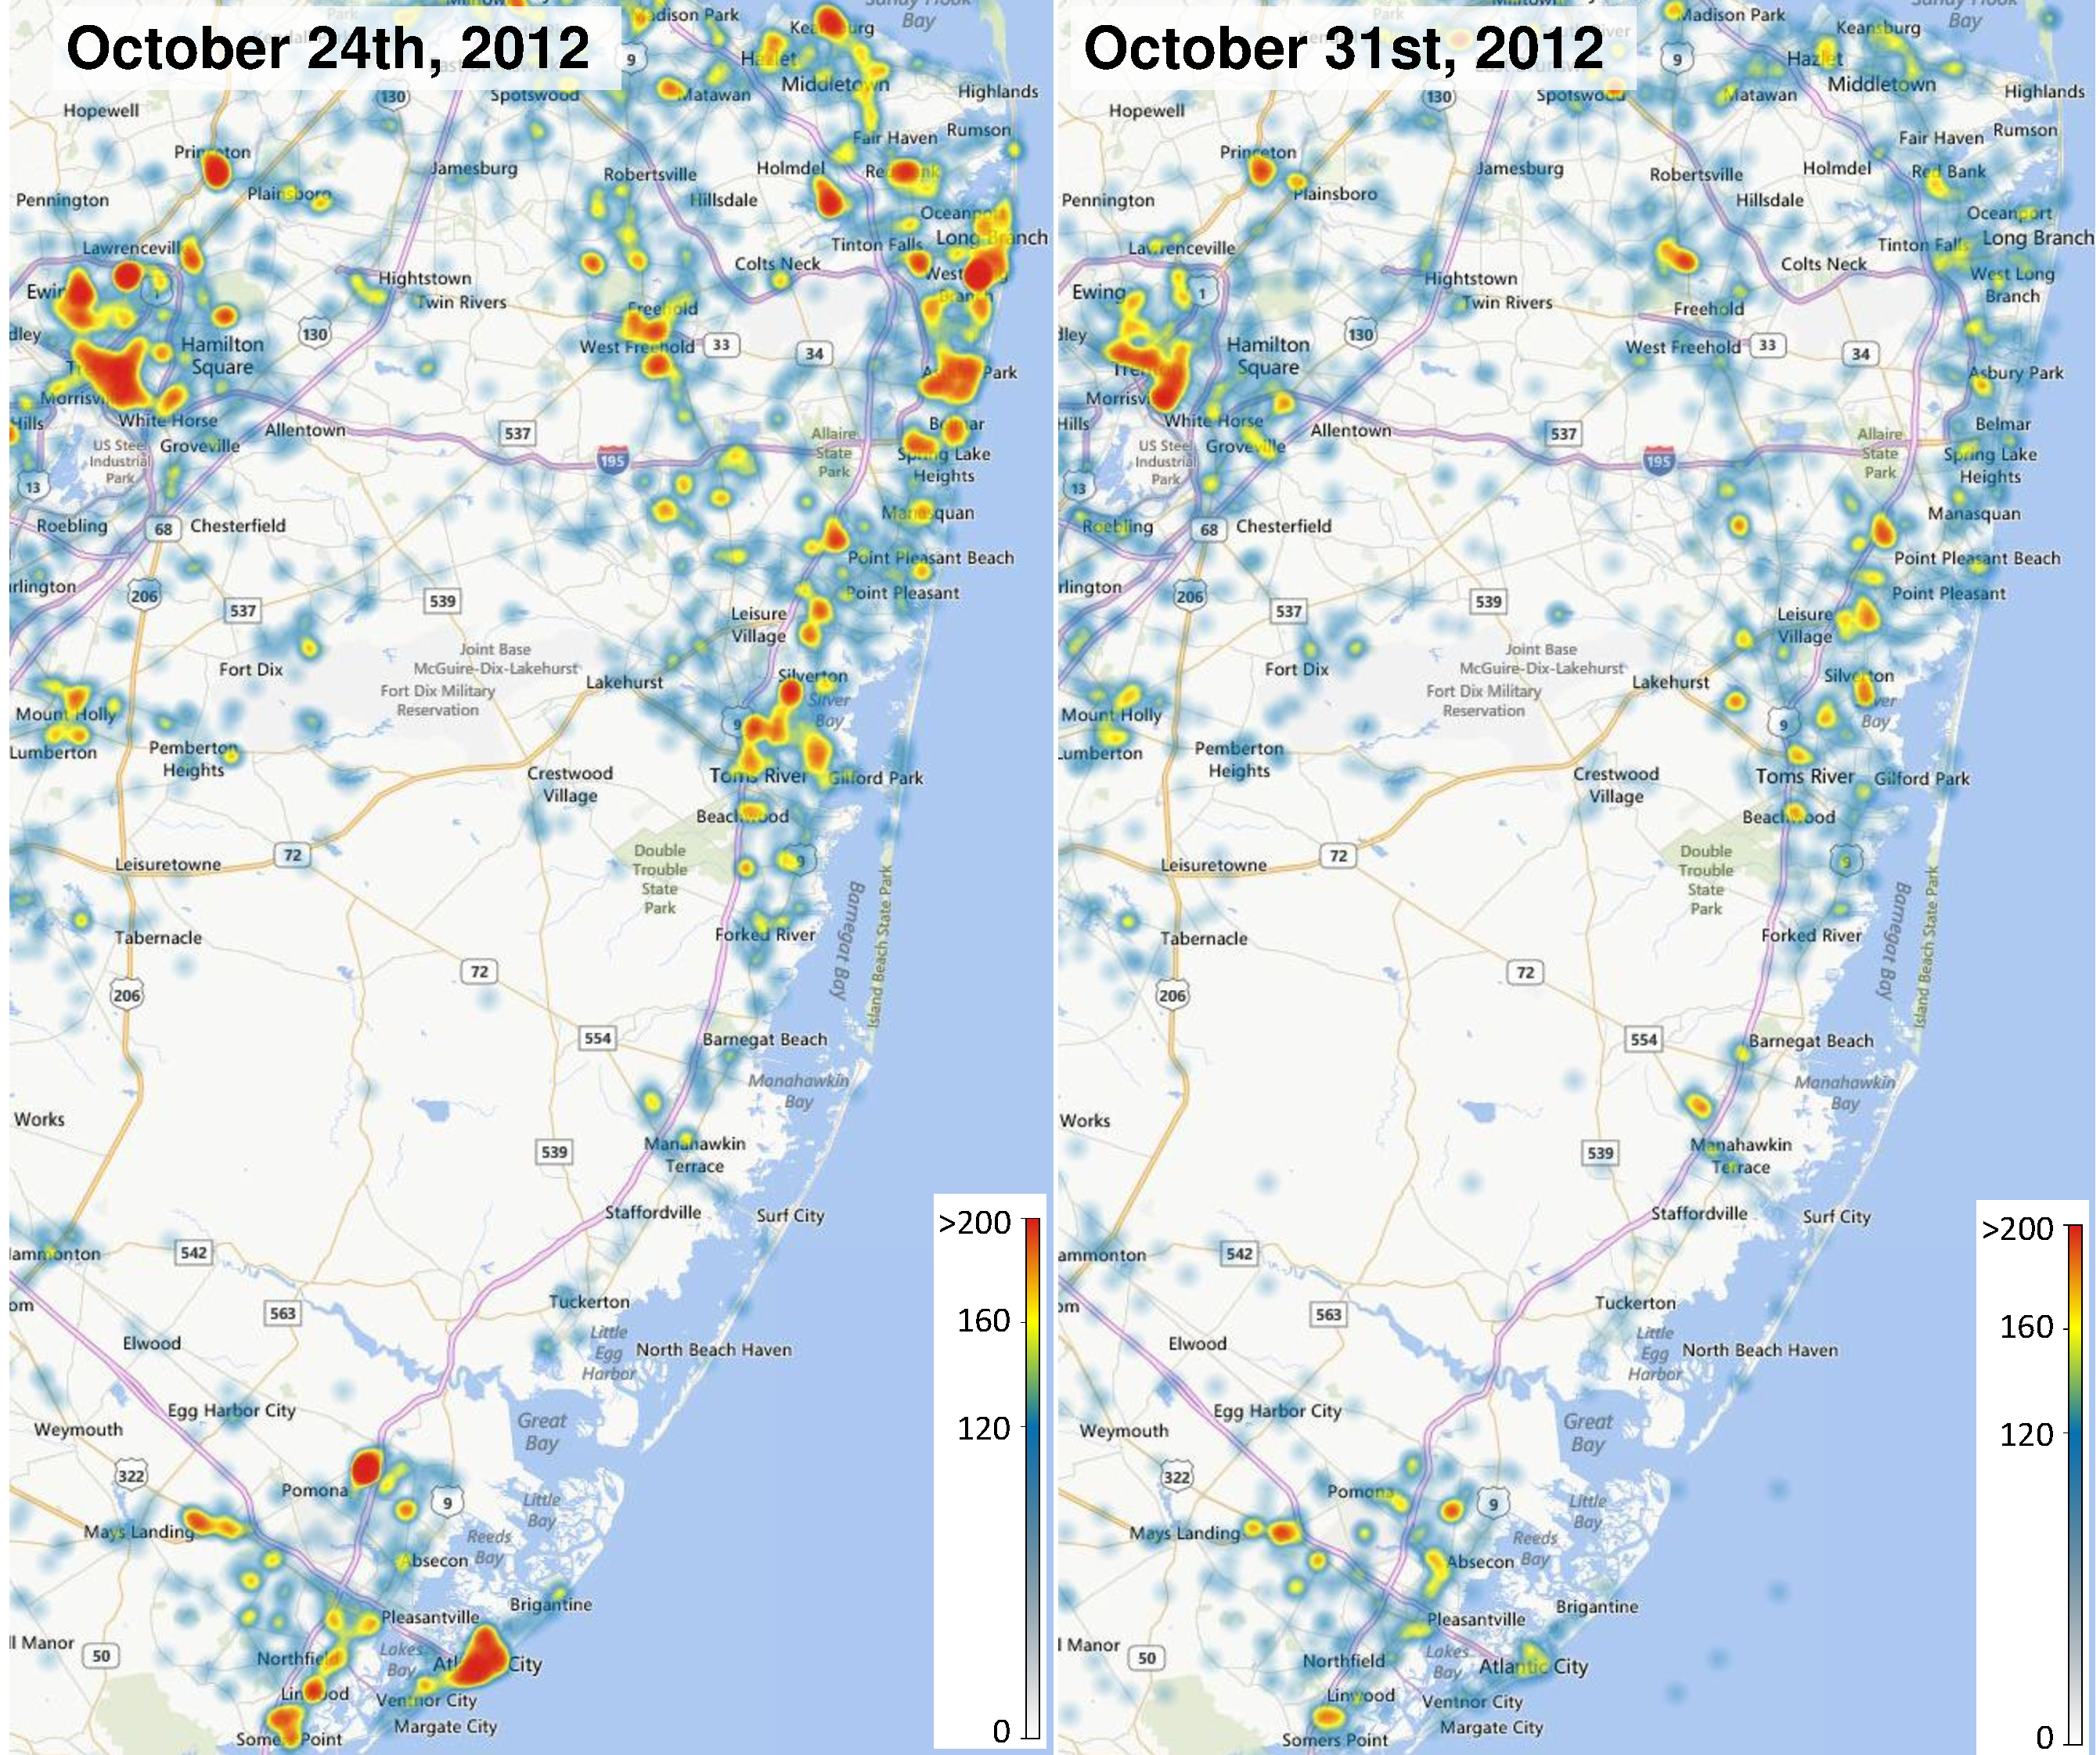
\includegraphics[width=1.0\linewidth]{Atlantic_Coast_v6}
\caption{Twitter user distribution on the eastern coast area in New Jersey, after the hurricane passed over the area on October 31st (Right). Previous distribution on October 24th is shown on the Left.}
\label{fig:atlantic_coast}
%\vspace{-0.4cm}
\end{figure}

Hurricane Sandy damaged not only New York City, but also the entire eastern coast area of New Jersey. 
Most cities in the area also announced evacuation orders on October 28th, 2012.
The distribution of Twitter users in the area from Atlantic City to the upper eastern shore area for two different dates are shown in Figure~\ref{fig:atlantic_coast}.
The heatmaps in Figure~\ref{fig:atlantic_coast} (Left) represent the previous normal situation of Twitter user distribution on October 24th and the heatmap (Right) shows the post distribution after Sandy passed over the area on October 31st.
As shown in the result, many hotspots are gone or diminished.
This situation shows that the number of Twitter users had significantly decreased after the hurricane damaged the area.
In fact, a huge number of homes were damaged or destroyed and a couple of million households lost power because of Hurricane Sandy~\cite{WKP:2012:EHS}.
In disaster management this type of visualization can support analysts estimating which areas were highly damaged and even which areas still need reconstruction.



%
%\begin{figure}[tb]
%\centering
%\includegraphics[width=0.8\columnwidth]{symbols}
%\caption{Standard symbols for infrastructures used in the paper~\cite{Robinson:2012:DMS}.}
%\label{fig:symbols}
%\vspace{-0.5cm}
%\end{figure}
%
%
%



